%! TEX root = ../barycenter.tex

% Discussions for metricized space of measures are available in the next chapter,
\begin{example}[A locally compact complete but not length space with a measure without barycenter]
	We endow the real line $\mathbb{R}$ with distance
	$d(x,y) = \phi(|x-y|)$ for $x,y \in \mathbb{R}$,
	where $\phi$ is a subadditive piecewise function defined by:
	$\phi(0) = 0$, $\phi(x) = x + 0.5$ for $ 0 <x <1$ and $\phi(x) = x+1$ for $x \geq 1$.
	This metric space is locally compact since all singletons are open, closed and compact.
	It is not a proper space since a closed ball with radius 1 contains
	infinitely many points while each point is an open set, so this ball is not compact.
	It follows that $(\mathbb{R}, d)$ is not a length space.
	We consider the probability measure $\mu :=\frac{1}{2}\delta_{-1}+ \frac{1}{2}\delta_1$ on $(\mathbb{R}, d)$.

	Define $f(x) := \int_{\mathbb{R}} d^2(x,y) \diff \mu(y) = \int_{\mathbb{R}} \phi^2(|x-y|) \diff \mu(y)$.
	We plots these two functions $\phi$ and $f$ below.
\begin{figure}[H]
	\centering
	\begin{minipage}{.49\textwidth}
		\centering
		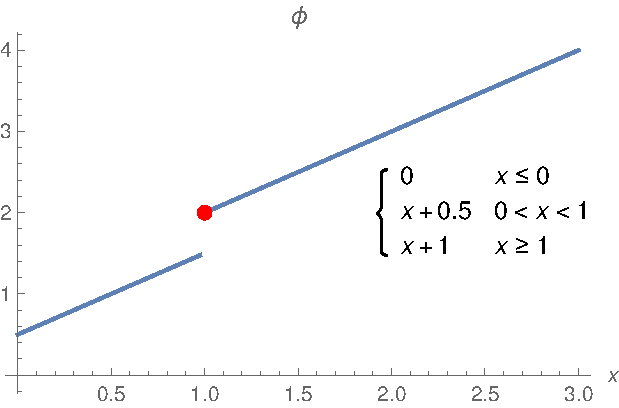
\includegraphics[height=.48\linewidth]{Chapters/example_phi.pdf}
		\caption{$d(x,y):=\phi(|x-y|)$}
	\end{minipage}
	\begin{minipage}{.49\textwidth}
		\centering
		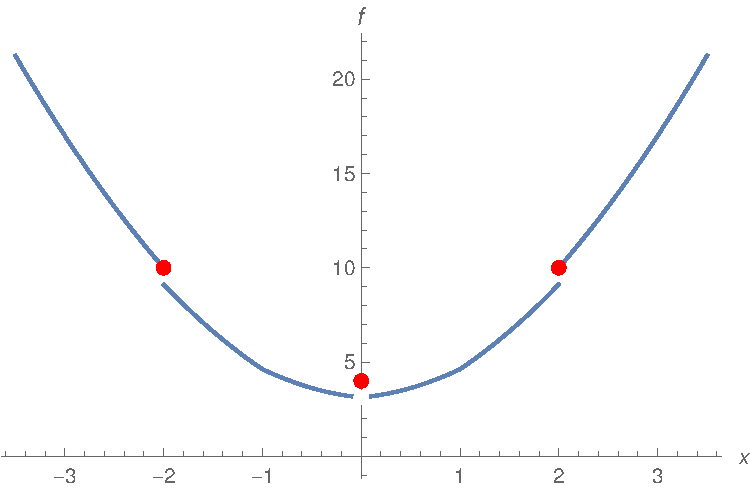
\includegraphics[height=.48\linewidth]{Chapters/example_f.pdf}
		\caption{$f(x) :=\int_{\mathbb{R}} d^2(x,y) \diff \mu(y)$}
	\end{minipage}
\end{figure}
	Red points are values of functions where they are discontinuous.
	Since $f$ has no minimal value, $\mu$ has no barycenter.
\end{example}

% \begin{rmk}
% 	An example of locally compact,
% 	separable and complete but not proper metric space is
% 	the real line $\mathbb{R}$ with distance $d(x,y)=\min\{|x-y|,1\}$.
% 	This metric space coincides with the restriction of Prokhorov metric
% 	to Dirac measures on $\mathbb{R}$.
% 	Recall that Prokhorov metric metricizes the weak convergence of Borel measures on $\mathbb{R}$.
% \end{rmk}

\begin{defn}
	A point \( z \in X \) is called a midpoint between points \( x \) and \( y \)
in a metric space \( ( X , d ) \) if \( d ( x , z ) = d ( z , y ) = \frac { 1 } { 2 } d ( x , y ) \).
\end{defn}

% Now let us focus on length space.
% $(E,d)$.  Recall that $(E,d)$ is path-connected by assumption.
We prove the following proposition as a method to construct counter-examples.

\begin{prop}[Barycenters and midpoints]
	\label{prop:barycenter_midpoint}
	For two points $x,y$ in a length space $(E,d)$,
	any barycenter of $\mu:=\frac{1}{2}\delta_x + \frac{1}{2}\delta_y$ 
	is a midpoint between $x$ and $y$
	and any such a midpoint is a barycenter.
	% That is to say, a barycenter $z$ satisfies $d(x,z)=d(z,y)=\frac{1}{2}d(x,y)$.
\end{prop}

\begin{proof}
	% There are two things to prove.

	If $z$ is a midpoint between $x$ and $y$,
	then it will attain the minimum in the following long inequality
	and thus, it is a barycenter
	\[
		d(x,y)^2 \leq \left(d(x,z) + d(z,y)\right)^2 \leq 2\left(d(x,z)^2+ d(z,y)^2\right).
	\]

	Now assume $z$ is a barycenter of $\mu:=\frac{1}{2}\delta_x + \frac{1}{2} \delta_y$.
	We denote by $\Gamma$ the set of all rectifiable curves from $x$ to $y$,
	by $L(\gamma)$ the length of rectifiable curve $\gamma$
	and by $\gamma_\frac{1}{2}$ the midpoint of $\gamma$ which exists from the continuity of length
	structure with respect to concatenation, see \Cref{rmk:curve_continuity_endpoints}.
	By definition of midpoint $\gamma_{\frac{1}{2}}$ and barycenter $z$,
	$L(\gamma_{[x, \gamma_\frac{1}{2}]}) = L(\gamma_{[\gamma_\frac{1}{2}, y]})$ for $\gamma \in \Gamma$ and
	\[
		d(x,z)^2 + d(z,y)^2 \leq {L(\gamma_{[x, \gamma_\frac{1}{2}]})}^2 + {L(\gamma_{[\gamma_\frac{1}{2}, y]})}^2=\frac{1}{2} {L(\gamma)}^2.
	\]
	Take the infimum over all $\gamma$ on the right hand side, we have $d(x,z)^2 + d(z,y)^2 \leq \frac{1}{2}d(x,y)^2$.
	This is equivalent to say that $z$ is a midpoint between $x$ and $y$.
\end{proof}


\begin{example}[No existence of barycenter in some length spaces]
	A locally compact complete length space is proper and hence guarantees the existence of barycenter.
	\begin{enumerate}
		\item Being a locally compact length space is not sufficient for the existence of barycenter.
		      Consider the unit disk without origin,
		      from physical intuition there is no barycenter for its uniform measure.
		      Or we can pick two center-symmetric points $x = - y$ and
		      take the measure $\frac{1}{2}\delta_x + \frac{1}{2}\delta_y$ as an example.
		\item Being a complete length space is not sufficient for the existence of barycenter.
			As we saw in \Cref{prop:barycenter_midpoint},
			if barycenters always exist then midpoints always exist.
		      However, in a complete length space this is the same as claiming that a shortest path always exists
		\cite[Theorem 2.4.16]{burago2001course}.
		      The idea behind the proof of this theorem
		      is to firstly construct our shortest path on rational points and then extend it
		      as a well-defined path by completeness and Lipschitz continuous of induced length structure with respect to rational points.
		      Moreover, we know that there exists a complete but not geodesic ``manifold''
		      in \underline{infinite dimension}, see \Cref{lem:infinite_not_geodesic_manifold} below.
	\end{enumerate}
\end{example}

\begin{defn}
	A length space is called geodesic if a shortest paths always exists.
	It is the same as saying that distance between two points is always realized by the length of some rectifiable curve.
\end{defn}

\begin{lem}
	\label{lem:infinite_not_geodesic_manifold}
	There exists a complete but not geodesic (infinite dimensional) Hilbert Riemannian manifold.
\end{lem}

One such example is the infinite dimensional ellipsoid in the Hilbert space $\ell^2$.
Let $(c_n)_{n \in \mathbb{N}^*}$ be a strictly decreasing sequence with a positive lower bound.
We define
\[
	E := \left\{ \left( x _ { 1 } , x _ { 2 } , \ldots \right) \in \ell^2 \mid \sum _ { n \in \mathbb { N }^* } \frac { x _ { n } ^ { 2 } } { c _ { n } ^ { 2 } } = 1 \right\}.
\]
We have met the space $E$ in \Cref{example:ellipsoid_subspaces},
but now we add a smooth structure to it.
The following proof is adapted from \cite[Example 5.1]{grossman1965hilbert}.

\begin{proof}
	Pick points $e=(c_1, 0,0,\ldots)$ and $-e=(-c_1, 0,0,\ldots)$,
	we aim to show that $e$ and $-e$ could not be connected by a minimizing geodesic.
	We regard $E$ as a smooth sub-manifold of $\ell^2 = \mathbb{R}^\mathbb{N}$.
	Hilbert Riemannian manifold theory is needed to justify the usage of term ``smooth'',
	but we leave the details about it out in this proof because
	our application of this theory is relatively plain.

	Define \( T: E \rightarrow E \) by \( T x = y \), where
	\begin{gather*}
		y _ { 1 } = x _ { 1 } , y _ { 2 } = 0 , y _ { i } = \frac{c_i}{c_{i-1}} x_{i-1} \text { for } i \geq 3, \\
		\sum_{n \in \mathbb{N}^*} \frac{y_i^2}{c_i^2} = \frac{x_1^2}{c_1^2} + 0 + \sum_{n \geq 3} \frac{x_{i-1}^2}{c_{i-1}^2}=1.
	\end{gather*}
	We shall show that any smooth curve from \( e\) to \( -e \) is mapped by \( T \)
	to another smooth curve which is strictly shorter than the original one.
	To justify this, recall that on (Hilbert) Riemannian manifold length structure is defined as arc-length integral.
	For a smooth curve $\gamma: [0,1] \rightarrow E$ with arc-length proportional parametrization,
	\[
		L(\gamma) := \int_{0}^{1} \| \gamma^\prime \| \diff \lambda \geq
		\int_{0}^{1} \| T^\prime(\gamma^\prime) \cdot \gamma^\prime \| \diff \lambda =: L(T \circ \gamma)
	\]

	Here the tangent map $T^\prime$ is an infinite dimensional matrix with
	diagonal $(1,0,{c_3}/{c_2}, \ldots)$.
	Since $\gamma^\prime$ is continuous,
	we are left with proving that in an open interval $\| \gamma^\prime \| > \| T^\prime(\gamma^\prime) \cdot \gamma^\prime \|$.
	Otherwise, $\gamma^\prime$ has only the first coordinate component on every open interval.
	Integrate $\gamma^\prime$ to get $\gamma \in \{ e, -e\}$.
	This is a contradiction.
\end{proof}

To get rid of Hilbert Riemannian manifold theory,
we prove a non-smooth version for this example.
We can show that $E$ with the metric inherited form $\ell^2$ is not a length space.
To explore more of this example,
we start to consider the intrinsic metric $\hat{d}$ on $E$.
% induced from inherited metric from $\ell^2$.

\begin{lem}
	\label{lem:ellipsoid_example_non_smooth}
	For $(E, d)$ in \Cref{example:ellipsoid_subspaces}, where $d$ is the inherited metric from $\ell^2$.
	Then there is, again, no shortest path $\gamma$ between two poles $e$ and $-e$
	so that $\hat{d}(e, -e) = L_d (\gamma)$.
\end{lem}

Since $ L_d = L_{\hat{d}}$,
this lemma tells that the length space $(E, \hat{d})$ is not geodesic.
In this sense, this lemma is a non-smooth version of the previous one.

\begin{proof}
	We start with a discussion of \underline{Lipschitz curves} from $[0,1]$ to $(E,d)$ connecting $e$ and $-e$.
	For a Lipschitz curve $\gamma$,
	one can define its derivative $\gamma^\prime: [0,1] \rightarrow \mathbb{R}^\mathbb{N}$ almost everywhere
	since each coordinate component of $\gamma$ is a Lipschitz function from $[0,1]$ to $\mathbb{R}$.
	Moreover, for a metric space $(E,d)$ our \Cref{defn:length_structure} of length structure is the same as
	the total variation of a Lipschitz function from $[0,1]$ to $\mathbb{R}^\mathbb{N}$.
	We can recover the classic arc-length integral formula (cf. \cite[Theorem 2.7.6]{burago2001course})
	\[
		L_d(\gamma |_{[s,t]}):= \int_s^t \| \gamma^\prime \| \diff \lambda
	\]
	by an argument similar to the proof of bounded variation formula
	\cite[Section 5.3]{Bogachev2007}:
	$\operatorname{V}(f, [s , t] )= \int_s^t |f^\prime| \diff \lambda$ whenever $f: [0,1] \rightarrow \mathbb{R}$ is absolutely continuous.

	A rectifiable curve $\gamma$
	always admits an arc-length proportional parametrization on $[0,1]$
	and its length does not depend on its parametrization
	(see \cite[Section 2.5.1]{burago2001course});
	with this parametrization
	it becomes a Lipschitz curve and $\| \gamma^\prime \| = L(\gamma)$ almost everywhere.

	We prove our lemma by contradiction and
	assume that there exists a minimal geodesic between $e$ and $-e$,
	then it could be realized by a Lipschitz curve.
	We claim that in $(E, \hat{d})$ arc-length variation has the same solution as energy variation
	over \emph{Lipschitz curves on $[0,1]$}:
	\begin{equation}
		\label{equa:energy_variation_in_E}
		\arg \min_{\gamma} L (\gamma) :=
		\arg \min_{\gamma} \int_{0}^{1} \| \gamma^\prime \| \diff \lambda =
		\arg \min_{\gamma} \int_{0}^{1} \| \gamma^\prime \| ^2 \diff \lambda
		\text{, where } \gamma \text{ is Lipschitz}.
	\end{equation}
	To justify \cref{equa:energy_variation_in_E},
	Cauchy-Schwarz inequality implies that
	solutions to energy variation should have arc-length proportional parametrizations.
	In this case, energy is exactly the square of the arc-length,
	so they attain their minima simultaneously.

	We show that there is no solution to this energy variational problem,
	and thus get a contradiction.
	Pick an integer $n \geq 2$,
	we modify $\gamma$ leaving $\gamma_k$ for $ k > n$ unchanged to lower the energy of $\gamma$.
	Define a continuous function
	$ c_{\gamma}(t) := \|(\frac{\gamma_1}{c_1}, \ldots, \frac{\gamma_n}{c_n} )\|$
	and an open subset $A: = c_\gamma^{-1}(0, \infty) \subset [0,1]$.
	Up to choosing a bigger $n$,
	we can assume that $ \gamma_{n-1} \neq 0$, so that $A$ is not empty.
	We modify $\gamma$ only on $A$ to define a curve $\eta$ in $E$,
	\[
		\eta(t) := (0,0,\ldots, c_n c_{\gamma}(t),\gamma_{n+1}(t),\ldots),\quad t \in A.
	\]
	Then on the non-empty open set $A \subset [0,1]$,
	\begin{align*}
		\| \gamma^\prime \|^2 - \| \eta^\prime \|^2 & =
		\|( \gamma_1^\prime,\ldots, \gamma_n^\prime )\|^2- (c_n c_\gamma^\prime)^2                         \\
		                                            & = \|( \gamma_1^\prime,\ldots, \gamma_n^\prime )\|^2-
		((\gamma_1^\prime, \ldots, \gamma_n^\prime) \cdot \frac{1}{c_\gamma}
		(\frac{c_n}{c_1} \frac{\gamma_1}{c_1}, \ldots, \frac{c_n}{c_n} \frac{\gamma_n}{c_n}))^2            \\
		                                            & \geq 0
	\end{align*}
	where we apply Cauchy-Schwarz and the assumption that $c_i$ is strictly decreasing.
	The previous inequality becomes strict in the set where $\| (\gamma_1^\prime(t), \ldots, \gamma_{n-1}^\prime(t)\| \ne 0$,
	which by our choice of $n$ is not negligible.
\end{proof}

\begin{rmk}
	In this non-smooth version counter-example, our proof heavily relies on the
	restriction to Lipschitz curves.
	% which enables us to define arc-length and energy variation in an analytic way.
	The good thing is that we can consider coordinate components for curves in $E \subset \mathbb{R}^\mathbb{N}$.
	Hence, we are allowed to apply classic non-smooth analysis for Lipschitz functions from $[0,1]$ to $\mathbb{R}$.
\end{rmk}
